\chapter{Results and analysis}
%Plan St 1
%In this chapter we showcase a series of results from the {\sc meqsilhouette} simulator. We begin with canonical simulations from the ISM, atmospheric and pointing error modules. Following this, we present the result of a typical calibration and imaging procedure in the presence of a variable source and a variable troposphere.
In this chapter we will showcase a series of results from the {\sc meqsilhouette} simulator in order to demonstrate it's capabilities and predictions.


\section{Canonical simulations}\label{sec:can_sim}
{\it Author's note: This section draws largely from the work of \citet{Blecher_2016}.}

\subsubsection{ISM variability and substructure}
%st 1
We remind the reader of the reproduction of the ISM-induced closure phase uncertainty result \citep{Ortiz_2016}, shown in Fig.~\ref{fig:substructure2}. To obtain this result we simulated 50 observations, each with an independent realisation of the ISM scattering screen. The success of the reproduction verifies a large section of the simulation software, including I/O, the interferometric and the ISM modules. 

%st1
Following the discussion on the ISM theory (section~\ref{sec:ism_scat}), we compare predictions of the ensemble-averaging regime, which consists of only a Gaussian convolution, and the average regime, which includes the presence of stochastic substructure. Note that the ensemble-average is invariant with time and would not bias the closure phase of a point-symmetric source.
%st1
\begin{quotation}  
``We present the results of a simulated observation of 10 minutes duration at 14:00 UTC on four consecutive days in Fig.~\ref{ISM_sequence}. To compare to published observations, we use the three-station EHT array consisting of the Submillimeter Telescope (SMT) in Arizona, the Combined Array for Research in Millimeter-wave Astronomy (CARMA) in California and the James Clerk Maxwell Telescope (JCMT) on Mauna Kea, Hawaii. The relative transverse velocity between the observer and scattering screen is set to $50~\rm{km\,s}^{-1}$ to be consistent with \citet{Ortiz_2016}. The source is a circular Gaussian with a $\rm{FHWM}=40$~$\mu$-arcsec, approximately the angular distance that a scattering screen would travel over $\sim 4$~days. The source size has been chosen such that it is consistent with the latest estimate of the size of Sgr~A$^\star$ at $230$~GHz \citep{Fish_2011}.  Closure quantities are model dependent and calculated as specified in \citet{Rogers_1995}, where the thermal noise was added based on the system equivalent flux density (SEFD) table in \citep{Lu_2014}.




Fig.~\ref{ISM_sequence} provides an example of closure phase and flux variability over a 4 day period using a static source. Accurate simulation of the ISM-induced closure phase variation is essential in order to make any inference on asymmetric, event-horizon scale structure \citep[e.g.][]{Fish_2016,Ortiz_2016}. This will become even more important as the EHT sensitivity increases by an order of magnitude in the near future when [phased ALMA is included in the array.]''
\citep{Blecher_2016} 
\end{quotation}

%to do : expand the analysis of the simulation out 
%st 1
This simulation clearly shows how the longest baselines are more sensitive to the refractive substructure, which in turn strengthens the challenge of imaging compact features and/or fine structure like the BH shadow. 


%%orbiting hot spot st1
Recalling the variability associated with Sgr~A* (section~\ref{sec:variability}), if the source has intrinsic spatial variability, e.g. an orbiting hotspot model \citep{Doeleman_2009} or jet shocks, this will increase ISM variability as the relative motion between source, screen and observer is increased \citep{Blecher_2016}. Although an orbiting plasma blob might be torn apart on sub-orbit timescales by differential rotation and the non-linear shear of the Magneto-Rotational Instability \citep[(MRI)][]{Balbus_1991}, this scenario becomes more of a physical possibility when resonant orbits are considered \citep{Brink_2015}. A resonant orbit occurs when the ratio of characteristic radial $\omega_r$ and longitudinal frequencies $\omega_\theta$ is a rational number $\omega_r/\omega_\theta = n/m$, where $n,m \in \mathbb{N}$. A hotspot in such an orbit could be stable against differential rotation and associated shearing. In the case of Sgr A*, the $1/2$ and $2/3$ resonances have  length scales of 41 and 55~$\mu$-arcsec respectively for a Schwarschild BH \citep{Brink_2015}, which is observable with the EHT. Also note that these resonant length scales are greater than $r_{\rm ref} \sim 10\ \mu$-arcsec and so the orbit would traverse independent refractive substructure fluctuations. This is relevant to methods like that demonstrated in \citet{Doeleman_2009} which rely on periodic closure phases. The periodic signal would exist (albeit altered by the ISM) but only on timescales less than $t_{\rm ref}$, assuming the orbiting body is unresolved.


%polarisation st 1 
Finally, we note that the ISM is polarisation invariant, hence the variability of polarisation ratios will not be biased by ISM scattering. Methods which use polarisation ratios \citep[e.g.][]{Johnson_2014} allows for valuable insight into how the source variability and ISM variability could be separated.



%st1
\begin{figure}[h!]
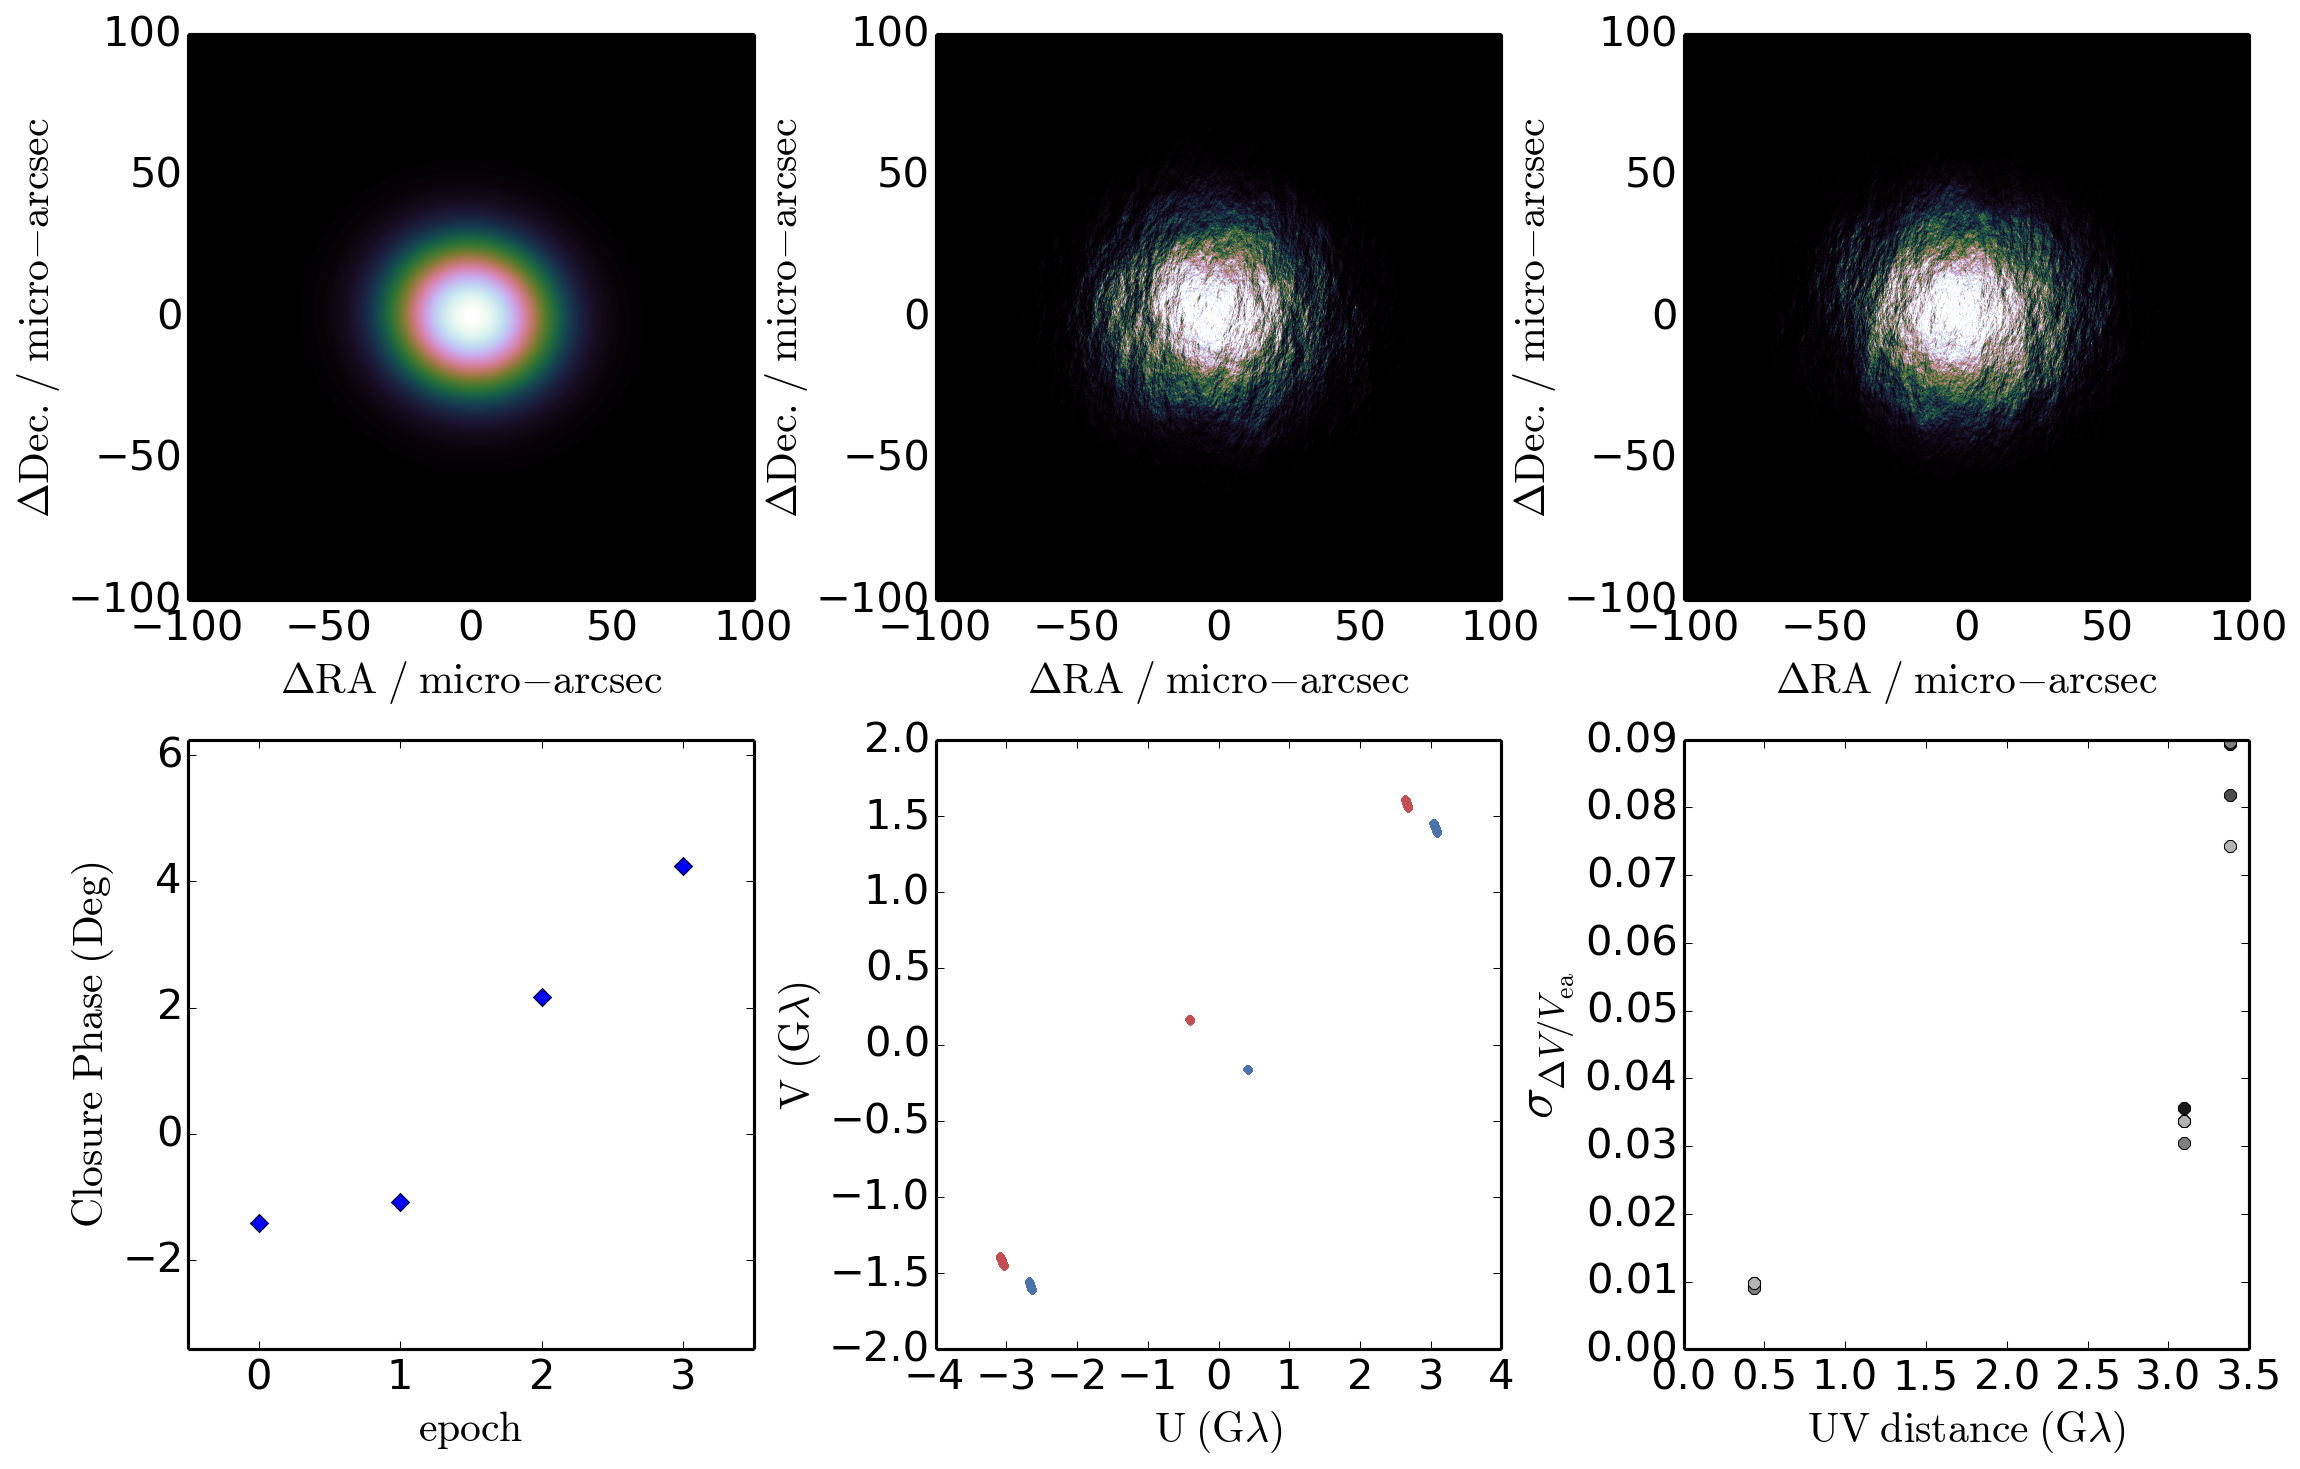
\includegraphics[width=\columnwidth]{Images/ism}
\caption{``An example simulation of ISM scattering towards Sgr~A$^{\star}$, observed with SMT-JCMT-CARMA.  The top panel, left to right, shows the original $\rm FWHM = 40$~$\mu$-arcsec Gaussian {\bf (top left)}, the simulated ISM scattered image on the first night {\bf (top middle)} and last night {\bf (top right)} of the observation, respectively.  The bottom panel, left to right,  shows the evolution of the 10 minute-averaged closure phase with epoch {\bf (bottom left)}, {\sl uv}-tracks for each night {\bf (bottom middle)} and the RMS fractional visibility amplitude differences $\sigma_{\Delta V /V_{\rm ea}}$ as a function of {\sl uv-}distance {\bf (bottom right)}. $ \Delta V= (|V_{\rm a}|-|V_{\rm ea}|)$, where $|V_{\rm a}|$ and $|V_{\rm ea}|$ are the simulated average and ensemble average visibility amplitudes respectively. Variations from the ensemble-average flux on the shortest baselines reveal total flux modulation while flux variations on longer baselines and non-zero closure phases track the fluctuations in substructure.''(Image and caption reproduced from \citet{Blecher_2016}) \label{ISM_sequence}%
}
\end{figure}

\subsubsection{Atmospheric transmission and scattering}

%st1
As described in section~\ref{sec:trop_imp}, the implementation of the tropospheric module is separated into mean and turbulent components. For the mean atmosphere, we simulate opacity, sky brightness temperature and time delay as a function of site weather, elevation angle and frequency. The most important climate parameters are precipitable water vapour column depth (PWV), ground temperature and ground pressure. The turbulent module simulates Guassian fluctuations in the time delay $\tilde{t}$ arriving at each station, where $\sigma(\tilde{t})$ is based on Kolmogorov turbulence on a two-dimensional scattering screen.


%Opacity + Brightness temperature st 1 - leave for now
The first atmospheric result we present are mean opacities and sky brightness temperatures for ALMA, the Submillimeter Array (SMA) and the South Pole Telescope (SPT) at 230~GHz, shown in Fig.~\ref{fig:mean_atm}. These sites were chosen as they are all considered excellent sites for sub-mm astronomy and form an essential part of the EHT. The PWV ranges used were taken from the 25th and 75th percentile data shown in \citet{Lane_1998} and is in good agreement with the measured opacities therein. %The ground% where I got the pressure/temp data from? I think it was SPT -lane 1998, ALMA - website/aatm defaults, SMA - site memo

%st 1
\begin{figure}[h!]
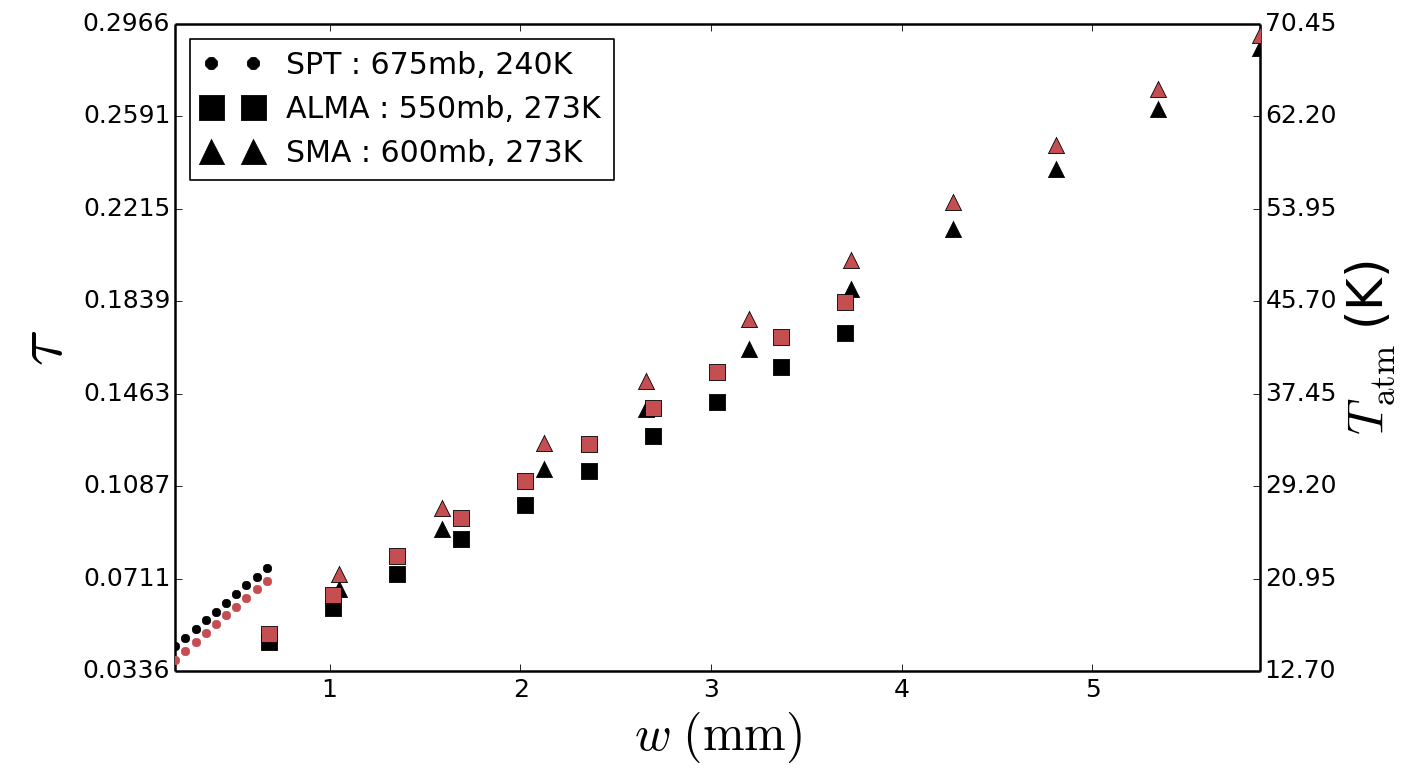
\includegraphics[width=1.\columnwidth]{Images/opacity}
\caption{``Simulated mean opacity (black) and sky brightness temperature (red) at $\nu =230$~GHz  for three typical ground pressures and temperatures over a typical PWV range \citep{Lane_1998} which approximately represent the sites of SPT (dots), ALMA (squares) and SMA (triangles). The legend shows the estimated input ground (pressure, temperature) parameters for each site.''(Image and caption reproduced from \citet{Blecher_2016})\label{fig:mean_atm}%
}
\end{figure}

%st 1 -a bit silly that I didnt do any 'bad' sites like PDBI or something like that
Immediately apparent is that the opacity and sky brightness temperature both exhibit linear relationships with respect to PWV content. Furthermore, opacity and sky brightness temperature are proportional to ground pressure and inversely proportional to the ground temperature \citep{Pardo_2001}. It is also clear that SPT has far less opacity, and a lower sky brightness temperature than ALMA and the SMA which are fairly similar. A comparison of the thermal receiver temperatures for the three sites  (ALMA$\sim262$~K,  SMA$\sim327$~K, SPT$\sim 255$~K) reveals that for the thermal noise contribution from the receiver is approximately an order of magnitude higher than sky brightness temperature. 



%Turbulent and mean delay st 1
Of vital importance to an interferometric site is atmospheric stability. An example of the effects of atmospheric transmission and scattering on the time delay $\tilde{t}$ at 230~GHz is shown as a function of observation time in Fig.~\ref{delay_plots}. Canonical values (see caption) were used for the weather parameters. It is apparent that the turbulent component is typically 3-4 orders of magnitude lower than the mean delay, even though the coherence time is on the order of seconds.


%st1
\begin{figure}[h!]
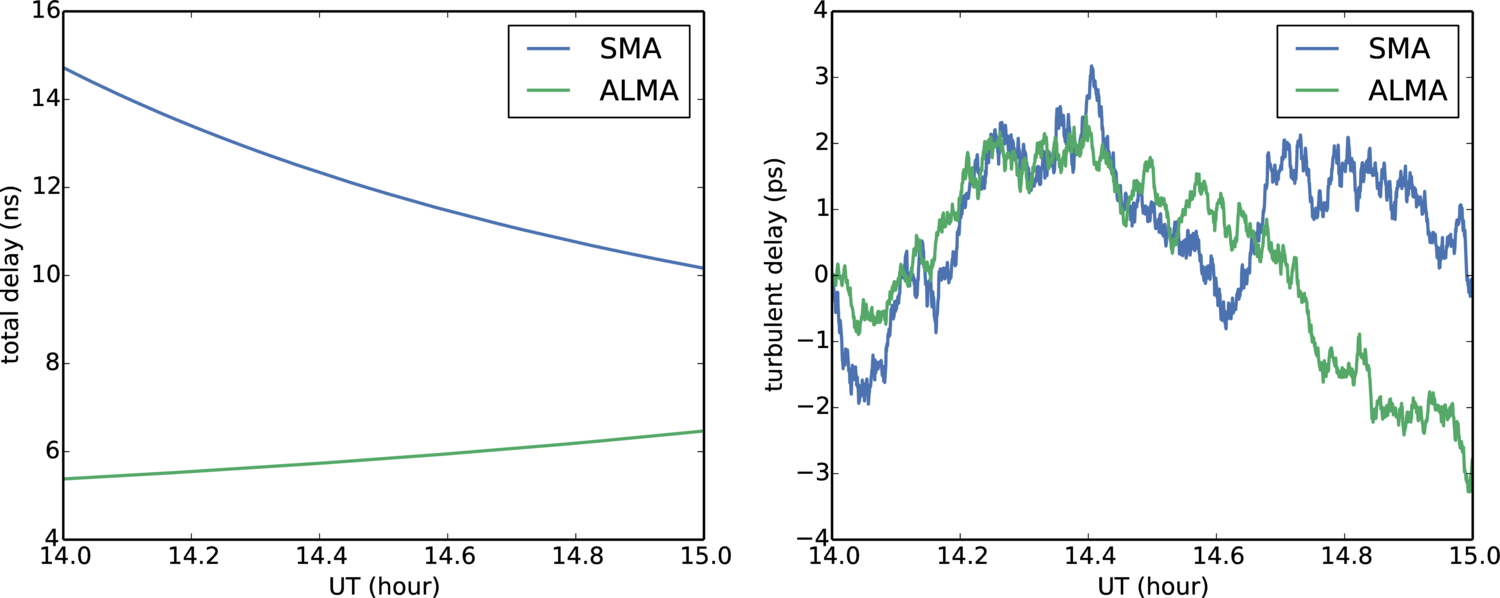
\includegraphics[width=\columnwidth]{Images/delays}
\caption{``Simulation of the total delay (left) and the turbulent atmospheric delay (right) for SMA (blue) and ALMA (green) sites towards Sgr~A$^\star$. Ground pressures and temperatures are the same as Fig.~\ref{fig:mean_atm}, precipitable water vapour above each station is set to $w=2$~mm, and the instantaneous zenith coherence time is set $T_0=10$~s for both stations. Note that all tropospheric parameters are, however, independently set. The conversion from time delay to phase at 230~GHz is $1$~rad~$=0.7$~ps.''(Image and caption reproduced from \citet{Blecher_2016})\label{delay_plots}%
}
\end{figure}



%Trop images
\begin{quotation}
``We now investigate the effect of the tropospheric module on image quality for various levels of calibration accuracy. We simulate the simple scenario of a sky model that consists of a 2.4~Jy point source at the phase centre, which is an approximate EHT-measured flux density of Sgr~A$^\star$ at 230~GHz. We assume a zenith phase coherence time of $t_0=10$~s above each station (however, each stations PWV can be independently simulated). We approximate the effect of imperfect calibration by adding a small fraction of the turbulent phase noise. For this example, we do not include the mean delay component, assuming it to be perfectly corrected for during the calibration. Imaging [is performed] using the two dimensional inverse fast Fourier transform''\\
\citep{Blecher_2016}
\end{quotation}

%Trop images
\begin{figure}[h!]
\includegraphics[width=\columnwidth]{Images/trop_images}
\caption{``The effect of residual troposphere phase noise on interferometric images of a point source observed for 12 hours at 230~GHz with 4~GHz bandwidth with the following array : SPT, ALMA, SMA, SMT, LMT and JCMT, assuming the same SEFDs as \protect\citet{Lu_2014} and an elevation limit of 15$^\circ$. For simplicity the weather parameters at each station were set to: coherence time $t_{\rm 0}=10$~sec; PWV depth $w=1$~mm; ground pressure $P=600$~mb; ground temperature $T =273$~K. {\bf Top left:} interferometric map with thermal noise only. {\bf Top right:} atmospheric attenuation and sky noise (due to non-zero opacity) with 1\% of the turbulent phase noise added. {\bf Bottom left:} as previous but with 3\% of turbulent phase contribution. {\bf Bottom right:} as previous but with 6\% turbulent phase contribution. The fractional turbulent phase contributions are illustrative of the effect of fringe-fitting errors. The black crosshairs indicate the original source position. ''(Image and caption reproduced from \citet{Blecher_2016}) \label{fig:trop_images}%
}
\end{figure}


%st 1 - attenuation of flux
Analysis of the images reveal increasing attenuation in the original peak, central flux due to the simulated residual calibration errors. In the calibration procedure, station gains cannot be solved for on arbitrarily short intervals as adequate SNR is needed to fringe-fit/self-calibrated. Aside from the fact that solutions are imperfect, within a given solution interval, there will also be a degree of uncalibrated turbulence-induced phase fluctuations.

Specifically, the flux of original central peak component is reduced to $76.5\%$ (attenuation only - not shown in plot), $75.1\%$ (1\% turbulence), 65.5\% (2\% turbulence) and  40.5\% (3\% turbulence). In the case of 3\% turbulence, the imaging artifact vertically below the source at 44.5\% of the original source flux becomes brighter than the corrupted source. 


%offset in original source st 1
Furthermore, there are slight offsets in the central peak flux from the original source position as shown by progressive movement away from the black crosshairs. This shift $\approx 5.6\ \mu$-arcsec at 3\% turbulence. 


%st 1
The residual calibration errors also distort the interferometric artifacts (as seen in the uncorrupted image), which result from inadequate sampling of the Fourier domain before imaging. This distortion causes a breakdown in image-plane deconvolution and source finding algorithms as the Point Spread Function (PSF) is difficult to subtract and the interferometric artefacts are difficult to distinguish from source structure. This further weakens the ability of such source finding algorithms to extract, with high fidelity, the BH shadow feature.


%Absence of blurring st 1 - but last sentence is dodgy, will change it in due course
There was no evidence of blurring or a loss of resolution in the simulated images. Blurring can result if the decoherence is considered as a function of baseline length, because longer baselines would be more decoherent and so their visibility amplitudes are effectively downweighted. For the EHT, as different stations experience completely independent phase fluctuations, the baseline length of the VLBI baselines will not be correlated with the magnitude of the decoherence. Alternatively, the blurring effect known to optical telescopes as 'seeing', which is induced by the overlaying of many speckled images of the source \citep{Narayan_1992} across the scattering disc, does not seem to occur in the interferometric image reconstruction. We suspect that this is due to destructive interference in the image domain from symmetrically distributed `speckles'.


%Incoherent closure phases.. This section is needed to link up to the discussion on closure phase uncertainty in the mm-VLBI section. Yep worth mentioning. but leave this 

%NON-CLOSING ERRORS
%Non-closing errors due to incoherent averaging - "no conjugates for triples" - possibly comes down to how one defines SNR. In the definition used in the literature we followed, they assumed only gaussian noise, which was not the case..A better definition would be to look at the distribution of a number of samples 
%maybe just a mention of how the closure phase uncertainty could change.

\subsubsection{Antenna pointing offset}

%mild intro



\begin{quotation}
``We investigate the effect of pointing errors on the 50~m (i.e. fully illuminated) Large Millimeter Array (LMT) dish configured in an eight station VLBI array. The LMT has been measured to have an absolute pointing accuracy of $\sigma_{\rm abs} = 1-3$~arcsec, where smaller offsets occur when observing sources closer to zenith, and a tracking pointing accuracy $\sigma_{\rm track} < 1$~arcsec\footnote{http://www.lmtgtm.org/telescope/telescope-description/}. We investigate the observational effect of these errors through three different pointing error models which explore different instructive and plausible scenarios. The LMT has been singled out as this may well serve as a reference station for the EHT array given its sensitivity and central geographic location. The source used is a circular Gaussian of characteristic size $\Theta_{\rm src}=50$ $\mu$-arcsec, located at the phase centre. For this investigation, as long as $\Theta_{\rm src} \ll \theta_{\rm PB}$, the exact structure of the source is unimportant. We approximate the LMT beam profile using an analytic WSRT beam model (equation~\ref{eq:wsrt_beam}) with a factor of two increase in the beam factor $C$ to take into account the increased dish size. [Hence] $C \approx 130$~GHz$^{-1}$. Note that the power beam $EE^H$ becomes $\cos^6$, resulting in a $\rm{FWHM} = 6.5 $~arcsec at 230 GHz.


We make use of the RMS fractional visibility amplitude error $\sigma_{\Delta V/V_0}$, where $V_{\rm PE}$ and $V_{0}$ are the visibility amplitudes with and without pointing errors respectively, and  $\Delta V = V_{\rm PE} - V_{0}$ . In Fig.~\ref{fig:pointing}, $\sigma_{\Delta V/V_0}$ is plotted against pointing error $\rho$ over the range $0 \le \rho \le 4.5$~arcsec.
\\
\citep{Blecher_2016}
\end{quotation}

%the different pointing models
In the first case we simulate, the most simple pointing model, a \emph{constant} pointing offset. For the second case, we simulate a smooth, \emph{sinusoidal} pointing error to replicate a tracking error. In the third case, we simulate \emph{stochastic} variability which replicates slewing from source to source/calibrator.  ''We simulate this \emph{stochastic variability} by re-sampling the pointing error every 10 minutes from a Gaussian of characteristic width equal to the quoted pointing error. We perform 50 realisations of the simulation for each pointing offset to generate reasonable uncertainties.''ees software package, such behaviour has been demonstrated to occur with the WSRT \citep{Smirnov_Calim_2011,Smirnov_2011c}. This is modeled as \emph{sinusoidal variability} with period sampled from a uniform distribution between 0.5 and 6 hours, and a peak amplitude $A_{\rho} = \sqrt{2} \sigma_{\rho}$ , where the factor $\sqrt{2}$ relates the peak amplitude to the RMS of a sinusoidal, zero-mean waveform. ''


\begin{quotation}
``In this simulation, we only consider LMT pointing errors due to its narrow primary beam and potential to be used as a reference station. However, the capability to simulate independent pointing errors for each station is available. In the case of a phased array, a pointing error simulation could be used to investigate the contribution of the pointing error to a variable phasing efficiency, which can be reasonably approximated by a scalar Jones matrix.''\\
\citep{Blecher_2016}
\end{quotation}


\begin{figure}[h!]
\includegraphics[width=\columnwidth]{Images/point_Crop}
\caption{``RMS relative amplitude error induced by pointing error with the 50~m (i.e. fully illuminated) LMT antenna as a function of pointing error offset $\rho$ at 230~GHz. We assume that these errors are degenerate or non-separable from the self-calibration/fringe-fitting model used. See text for the description of the three models used. This simulation capability enables constraints on the magnitude of pointing-induced errors given a particular pointing calibration strategy.''(Image and caption reproduced from \citet{Blecher_2016})\label{fig:pointing}%
}
\end{figure}
\

\begin{quotation}
``Visibility amplitude errors due to antenna pointing error has been investigated for the $50$~m  LMT dish operating at $230$~GHz. In Fig.~\ref{fig:pointing}, we show that pointing errors associated with frequent phase centre switching (stochastic variability) could introduce a RMS fractional amplitude error $\sigma_{\Delta V/V_0} \sim 0.1 - 0.4$ for an absolute pointing accuracy  $\sigma_{\rm abs} \sim 1-3$~arcsec. In contrast, tracking errors are less problematic with $\sigma_{\Delta V/V_0} \le 0.05$ for a tracking accuracy  $\sigma_{\rm track}<1$~arcsec. The case of a constant error pointing model is comparable to that of the `slow variability' case. If the gain error is non-separable from the calibration model used, it could be interpreted as intrinsic variability, substructure and/or increased noise. If unaccounted for, this effect has the potential to limit the dynamic range of mm-VLBI images. Further tests to constrain the pointing uncertainties of EHT stations will lead to more accurate interferometric simulations and hence the overall impact on black hole shadow parameter estimation. Here we demonstrate the capability to incorporate a range of plausible pointing error effects into a full simulation pipeline. For future observations at 345~GHz, these effects will be even more pronounced, given the narrower primary beam.\\
\citep{Blecher_2016}
\end{quotation}


%\subsubsection{Performance?}
%Performance/speed

%\section{Fringe-fitting test}
%leave until done
%First we fringe fit and image a stationary point source and compare to the result in Fig.~\ref{fig:trop_images}. 
% In an upcoming paper, we perform a systematic exploration of the turbulent tropospheric effects on the accuracy of fringe-fitting algorithms/strategies, through use of an automated calibration procedure and including the added complexity of a time-variable source.

